Ξεκινώντας με την επίλυση της κατάστασης του οχήματος, αξιοποιούμε τα δεδομένα ταχύτητας $U_{\hat{X}}(s)$ του οχήματος σε συνδυασμό με τη γεωμετρία της πίστας.

Οι επιταχύνσεις και ο ρυθμός εκτροπής μετρώνται με επιταχυνσιόμετρα και γυροσκόπια αντίστοιχα καθώς αποτελούν προσιτό πακέτο αισθητήρων με τα οποία είναι εξοπλισμένα πλέον τα περισσότερα αγωνιστικά οχήματα. Ωστόσο, στην παρούσα εργασία θα προσεγγίσουμε αυτά τα μεγέθη μέσω της τροχιάς του οχήματος.\\[5pt]

Η τροχιά του οχήματος εκφράζεται με καμπυλόγραμμες συντεταγμένες (curvilinear), όπου η πίστα αποτυπώνεται ως μία αλληλουχία καμπών σταθερής ακτίνας ή ευθειών (\cref{fig:barcelonaCurvilinear}), σχηματίζοντας τελικά μία περιγραφή της μορφής $R(s)$.

\begin{figure}[ht!]
    \begin{center}
        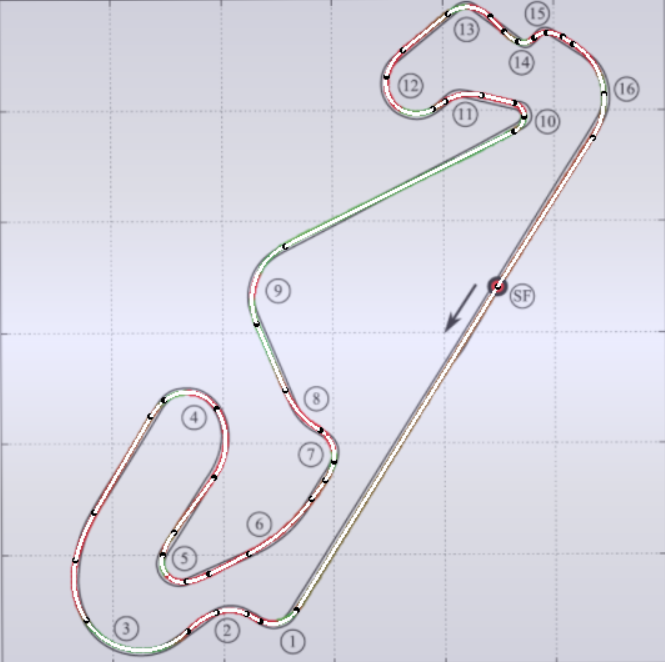
\includegraphics[width=0.6\textwidth]{figures/barcelona_curvilinear2.png}
    \end{center}
    \caption{Αποτύπωση πίστας \textit{Circuit de Barcelona - Catalunya} σε καμπυλόγραμμες συντεταγμένες.}
\label{fig:barcelonaCurvilinear}.
\end{figure}

Η διαμήκης επιτάχυνση κατά μήκος της τροχιάς υπολογίζεται με παραγώγιση της σειράς της ταχύτητας $U_{\hat{X}}(s)$ με κεντρικές πεπερασμένες διαφορές. Σημειώνεται πως στην υλοποίηση, το πεδίο της ταχύτητας εξομαλύνθηκε με μέθοδο Savitzky \& Golay \cite{SavitzkyGolay1964}, για την αποφυγή διάδοσης θορύβου λόγω της αριθμητικής παραγώγισης.

\begin{equation}
    \alpha_{\hat{X}}(s_i) = \dfrac{U_{\hat{X}}(s_{i+1}) - U_{\hat{X}}(s_{i-1})}{2h}
    \label{eq:finDiffAx}
\end{equation}

Και η πλευρική επιτάχυνση εκφρασμένη στο κινούμενο σύστημα αξόνων $\hat{X}\hat{Y}$ δίνεται στην \cref{eq:kinematicAy}. Εξ'ορισμού, η συνιστώσα $U_{\hat{Y}} = 0$ καθώς το σύστημα ορίζεται με τον άξονα $\hat{X}$ στη διεύθυνση της ταχύτητας του κέντρου μάζας.

\begin{equation}
    \alpha_{\hat{Y}} = \dfrac{dU_{\hat{Y}}}{dt} = 0
    \label{eq:kinematicAy}
\end{equation}


Για τον υπολογισμό του ρυθμού εκτροπής θεωρούνται συνθήκες μόνιμης κατάστασης. Στην πράξη, στην είσοδο και έξοδο της στροφής το όχημα βρίσκεται σε μεταβατική κατάσταση, ωστόσο, παραδεχόμαστε πως αυτό το μεταβατικό τμήμα συμβαίνει σε μικρό ποσοστό του γύρου και δεν επηρεάζει σημαντικά τη συνολική εξέλιξη της θερμοκρασίας και της φθοράς. Επομένως, για συνθήκες μόνιμης κατάστασης, ο ρυθμός εκτροπής είναι:

\begin{equation}
    \dot{\psi}(s) = \dfrac{U_{\hat{X}}(s)}{R(s)}
    \label{eq:steadyStateYawRate}
\end{equation}
